\documentclass[../main.tex]{subfiles}
\graphicspath{{\subfix{../images/}}}
\begin{document}
	Given the velocity field: $\un{v}=xt\un{i} + \un{j}$.
	Determine:
	\begin{enumerate}
		\item The stream lines
		\item The path line (Parametric and explicit)
		\item The streak lines (Parametric and explicit)
	\end{enumerate}

	\subsection{Stream lines}
	\begin{equation*}
		\frac{dx}{u} = \frac{dy}{v} => \frac{dx}{xt} = \frac{dy}{1}
	\end{equation*}

	\begin{align*}
		\int \frac{dx}{x} &= \int t dy \\
		ln(x) &= ty + c_1 \\
		x &= e^{ty + c_1} = C_2 e^{ty}
	\end{align*}
	\begin{figure}[ht]
		\centering
		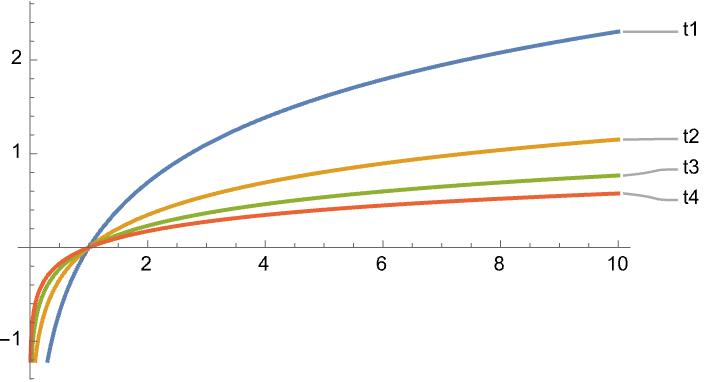
\includegraphics[width=7cm]{stream-line-figure}

		\label{fig:stream}
		\caption{Stream Lines at different times}
	\end{figure}

	\subsection{Path Lines}
	\textbf{Parametric form:}
	\begin{align*}
		\frac{dX}{dt} &= Xt \\
		\int \frac{dX}{x} &= \int t dt \\
		ln(X) &= \frac{t^2}{2} + C_3 \\
		X &= C_4 e^{\frac{t^2}{2}}
	\end{align*}
	At $t=0$, $X=X_0$. Therefor $C_4 = X_0$
	\begin{equation}
		X = X_0 e^{\frac{t^2}{2}}
	\end{equation}
	Calculating the Y component:
	\begin{align*}
		\frac{dY}{dt} &= 1 \\
		\int dY &= \int dt \\
		Y &= t + C_5 
	\end{align*}
	At $t=0$, $Y=Y_0$. Therefor $C_5 = Y_0$
	\begin{equation}
		Y = t + Y_0
	\end{equation}
	\textbf{Explicit Form:}
	Eliminate t, $t=Y-Y_0$
	\begin{equation*}
		X = X_0 e^{0.5 (Y - Y_0)^2}
	\end{equation*}
	\begin{equation*}
		\ln(\frac{X}{X_0}) = \frac{1}{2} (Y-Y_0)^2
	\end{equation*}
	\begin{equation}
		Y = Y_0 + \sqrt{2 \ln(\frac{X}{X_0})}
	\end{equation}

	\begin{figure}[ht]
		\centering
		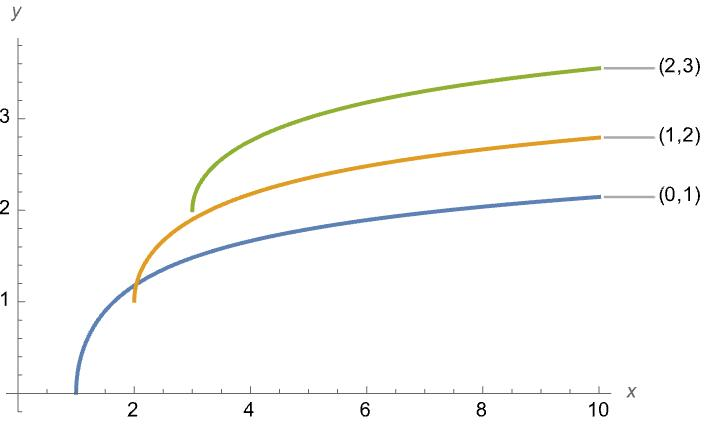
\includegraphics[width=7cm]{path-lines}

		\label{fig:pathline}
		\caption{Path lines for different starting points}
	\end{figure}
	\subsection{Streak lines}
	\textbf{Parametric Form:}
	Calculating the X component:
	\begin{align}
		\label{eq:22}
		X &= X_0 e^{0.5 t^2} \\
		X^{*} &= X_0 e^{0.5 \tau ^2} \\
		\label{eq:24}
		X_0 &= X^{*} e^{-0.5 \tau ^2}
	\end{align}
	Substitute (\ref{eq:24}) into (\ref{eq:22}). Resulting in:
	\begin{equation}
		\label{eq:25}
		X = X^{*} e^{0.5(t^2 - \tau ^2)}
	\end{equation}
	Calculating the Y component:
	\begin{align}
		\label{eq:26}
		Y &= Y_0 + t \\
		Y^{*} &= Y_0 + \tau \\
		\label{eq:27}
		Y_0 &= Y^{*} - \tau
	\end{align}
	Substitute (\ref{eq:26}) into (\ref{eq:27}). Resulting in:
	\begin{equation}
		\label{eq:29}
		Y = Y^{*} + t - \tau
	\end{equation}

	\textbf{Explicit Form:}
	Using  (\ref{eq:25}) to eliminate $\tau$:
		\begin{equation*}
		\ln(\frac{X}{X^*}) = \frac{1}{2} (t^2 - \tau ^2)
		\end{equation*}
		\begin{equation}
			\label{eq:30}
			\tau = \sqrt{t^2 - 2 \ln(\frac{X}{X^*})}
		\end{equation}

		Substitute (\ref{eq:30}) into (\ref{eq:29}), which results in the explicit form:
		\begin{equation}
			Y = Y^{*} + t - \sqrt{t^2 - 2 \ln(\frac{X}{X^*})}
		\end{equation}
\end{document}
